%input macros (i.e. write your own macros file called MacroFile1.tex)
%\newcommand{\PdfPsText}[2]{
  \ifpdf
     #1
  \else
     #2
  \fi
}

\newcommand{\IncludeGraphicsH}[3]{
  \PdfPsText{\includegraphics[height=#2]{#1}}{\includegraphics[bb = #3, height=#2]{#1}}
}

\newcommand{\IncludeGraphicsW}[3]{
  \PdfPsText{\includegraphics[width=#2]{#1}}{\includegraphics[bb = #3, width=#2]{#1}}
}

\newcommand{\InsertFig}[3]{
  \begin{figure}[!htbp]
    \begin{center}
      \leavevmode
      #1
      \caption{#2}
      \label{#3}
    \end{center}
  \end{figure}
}


%%% Local Variables: 
%%% mode: latex
%%% TeX-master: "~/Documents/LaTeX/CUEDThesisPSnPDF/thesis"
%%% End: 


 \documentclass[oneside,12pt]{Classes/CUEDthesisPSnPDF}


\ifpdf
    \pdfinfo { /Title  (NGO Report)
               /Creator (TeX)
               /Producer (pdfTeX)
               /Author (Kartikeya Gupta)
               /CreationDate (D:20030101000000)  %format D:YYYYMMDDhhmmss
               /ModDate (D:20030815213532)
               /Subject (Synergy Sansthan)
               /Keywords (HUL265)}
    \pdfcatalog { /PageMode (/UseOutlines)
                  /OpenAction (fitbh)  }
\fi

\title{NGO report: Synergy Sansthan\\[1ex]
        HUL265: Theories of Personality}

\ifpdf
  \author{\href{mailto:cs1130231@iitd.ac.in}{Kartikeya Gupta}}
  \collegeordept{\href{http://www.cse.iitd.ac.in}{2013CS10231}}
  \university{\href{http://www.iitd.ac.in}{IIT Delhi}}
% insert below the file name that contains the crest in-place of 'UnivShield'
  \crest{
\includegraphics[width=40mm]{iitd_logo}}
\else
  \author{Kartikeya Gupta}
  \collegeordept{Department of Engineering}
  \university{University of Cambridge}
% insert below the file name that contains the crest in-place of 'UnivShield'
  \crest{
\includegraphics[bb = 0 0 292 336, width=30mm]{iitd_logo}}
\fi
%
% insert below the file name that contains the crest in-place of 'UnivShield'
% \crest{\IncludeGraphicsW{UnivShield}{40mm}{14 14 73 81}}
%
%\renewcommand{\submittedtext}{change the default text here if needed}
\degree{HUL265 Theories of personality}
\degreedate{}

% turn of those nasty overfull and underfull hboxes
\hbadness=10000
\hfuzz=50pt

% Put all the style files you want in the directory StyleFiles and usepackage like this:
% \usepackage{StyleFiles/watermark}

% Comment out the next line to get single spacing
\onehalfspacing

\begin{document}

%\language{english}

% A page with the abstract on including title and author etc may be
% required to be handed in separately. If this is not so, then comment
% the below 3 lines (between '\begin{abstractseparte}' and 
% 'end{abstractseparate}'), normally like a declaration ... needs some more
% work, mind as environment abstracts creates a new page!
% \begin{abstractseparate}
%   
% Thesis Abstract -----------------------------------------------------


%\begin{abstractslong}    %uncommenting this line, gives a different abstract heading
\begin{abstracts}        %this creates the heading for the abstract page

The goal is to do a systematic analysis of the work performed by a NGO of our choice. We have to analyze the work it does, the change it is bringing about by talking to the people associated with the NGO directly and indirectly both.

The NGO I have chosen is Synergy Sansthan. I have chosen it because I had done an internship there in December. Through the internship, I was able to closely witness the actual working of the NGO and understand it better.

\end{abstracts}
%\end{abstractlongs}


% ----------------------------------------------------------------------


%%% Local Variables: 
%%% mode: latex
%%% TeX-master: "../thesis"
%%% End: 

% \end{abstractseparate}




% Using the watermark package which is in StyleFiles/
% and to remove DRAFT COPY ONLY appearing on the top of all pages comment out below line
%\watermark{DRAFT COPY ONLY}


\maketitle

%set the number of sectioning levels that get number and appear in the contents
\setcounter{secnumdepth}{3}
\setcounter{tocdepth}{3}

\frontmatter % book mode only
\pagenumbering{roman}
% % Thesis Dedictation ---------------------------------------------------

\begin{dedication} %this creates the heading for the dedication page

I would like to dedicate this thesis to my loving parents ...

\end{dedication}

% ----------------------------------------------------------------------

%%% Local Variables: 
%%% mode: latex
%%% TeX-master: "../thesis"
%%% End: 

% % Thesis Acknowledgements ------------------------------------------------


%\begin{acknowledgementslong} %uncommenting this line, gives a different acknowledgements heading
\begin{acknowledgements}      %this creates the heading for the acknowlegments


And I would like to acknowledge ...


\end{acknowledgements}
%\end{acknowledgmentslong}

% ------------------------------------------------------------------------

%%% Local Variables: 
%%% mode: latex
%%% TeX-master: "../thesis"
%%% End: 


% Thesis Abstract -----------------------------------------------------


%\begin{abstractslong}    %uncommenting this line, gives a different abstract heading
\begin{abstracts}        %this creates the heading for the abstract page

The goal is to do a systematic analysis of the work performed by a NGO of our choice. We have to analyze the work it does, the change it is bringing about by talking to the people associated with the NGO directly and indirectly both.

The NGO I have chosen is Synergy Sansthan. I have chosen it because I had done an internship there in December. Through the internship, I was able to closely witness the actual working of the NGO and understand it better.

\end{abstracts}
%\end{abstractlongs}


% ----------------------------------------------------------------------


%%% Local Variables: 
%%% mode: latex
%%% TeX-master: "../thesis"
%%% End: 


\tableofcontents
\listoffigures
\printnomenclature  %% Print the nomenclature
% \addcontentsline{toc}{chapter}{Nomenclature}

\mainmatter % book mode only
%%% Thesis Introduction --------------------------------------------------
\chapter{Introduction}
\ifpdf
    \graphicspath{{Introduction/IntroductionFigs/PNG/}{Introduction/IntroductionFigs/PDF/}{Introduction/IntroductionFigs/}}
\else
    \graphicspath{{Introduction/IntroductionFigs/EPS/}{Introduction/IntroductionFigs/}}
\fi

Synergy organization started its work in a group since 2004 in Indore Madhya Pradesh and was registered on May 15, 2006. The early members who were mainly youngsters started working among the slums of Indore city. Later on it was felt by the youth to form such group, which can perform better in the fields of social services giving special focus to awareness in the slum area like AIDS, hygiene, immunization and education. Thus the name ``SYNERGY'' was carved out of the experience from the works through participatory action and energetic. \newline
Synergy is the group of some devoted youth who are committed to serve the poverty stricken and vulnerable people with special attention to empower women, children and local self-governance. In the fast changing socio-economic condition, social security becomes an issue of major concern. With rapid deterioration in moral, traditional and cultural values, changing climatic conditions due to environmental degradation and frequent natural disasters, the reality is changing rapidly. The rise in crime rate, number of orphanages, old age homes etc. are the result of waning human empathy. So in this situation Synergy believes in creating a society that is sustainable and is free from exploitation of humans and natural resources and by proving equal opportunity to the marginalized, poor, women and children to develop. It also makes efforts in making a society with sustainable human development and building capacity, sharing common vision of institution and nation building and reinforcing human development endeavors for over all progress of mankind. Synergy also believes in participatory action at the community level.
%%% ----------------------------------------------------------------------


%%% Local Variables: 
%%% mode: latex
%%% TeX-master: "../thesis"
%%% End: 

% \pagebreak[4]
% \hspace*{1cm}
% \pagebreak[4]
% \hspace*{1cm}
% \pagebreak[4]

\chapter{Synergy Sansthan}
\ifpdf
    \graphicspath{{Chapter1/Chapter1Figs/PNG/}{Chapter1/Chapter1Figs/PDF/}{Chapter1/Chapter1Figs/}}
\else
    \graphicspath{{Chapter1/Chapter1Figs/EPS/}{Chapter1/Chapter1Figs/}}
\fi

\section{Founders}
\begin{itemize}
	\item \textbf{Mr. Ajay Pandit} \newline
		Mr Ajay Pandit, founder member and Executive Secretary of Synergy Sansthan, belongs to a farmer family. He is 30 year old. His education is MSW, Diploma in Disaster Management \& fellow of National child right fellowship of CRY. Mr. Ajay is also conducting various study like that Process documentation of ``technically support system for SSA'' of MV foundation, Education Micro Plan for Aide et Action etc. He has been working in the voluntary sector for the last 6 years. In the year 2006 he started the activities under the banner of Synergy Sansthan in block Timarni of Harda district in Madhya Pradesh.
	\item \textbf{Mr. Vimal Jat} \newline
		Mr. Vimal Jat, 27 is the President of Synergy Sansthan. His educational background is MSW. He has over 5 years of experience in the social sector. His main areas of focus with Synergy Sansthan are assessing the overall working of different bodies and procuring funds from other NGOs and individuals.
	\item \textbf{Mr. Vishnu Jaiswal} \newline
		Mr. Vishnu Prasad Jaiswal, 28 is the Vice President of Synergy Sansthan. His educational background is MSW,  MBA. He has a lot of experience in the social sector. He belongs to an agriculture based family. He is associated with the child line team of Synergy Sansthan and monitors their activities closely.
\end{itemize}

% Here is an equation\footnote{the notation is explained in the nomenclature section :-)}:
% \begin{eqnarray}
% CIF: \hspace*{5mm}F_0^j(a) &=& \frac{1}{2\pi \iota} \oint_{\gamma} \frac{F_0^j(z)}{z - a} dz
% \end{eqnarray}
% \nomenclature[zcif]{$CIF$}{Cauchy's Integral Formula}                                % first letter Z is for Acronyms 
% \nomenclature[aF]{$F$}{complex function}                                                   % first letter A is for Roman symbols
% \nomenclature[gp]{$\pi$}{ $\simeq 3.14\ldots$}                                             % first letter G is for Greek Symbols
% \nomenclature[gi]{$\iota$}{unit imaginary number $\sqrt{-1}$}                      % first letter G is for Greek Symbols
% \nomenclature[gg]{$\gamma$}{a simply closed curve on a complex plane}  % first letter G is for Greek Symbols
% \nomenclature[xi]{$\oint_\gamma$}{integration around a curve $\gamma$} % first letter X is for Other Symbols
% \nomenclature[rj]{$j$}{superscript index}                                                       % first letter R is for superscripts
% \nomenclature[s0]{$0$}{subscript index}                                                        % first letter S is for subscripts

\section{Vision}
``Promoting intensive participatory process of natural resources development and local institution development. Particular emphasis on unreached, under reached area and women, child, poor and marginalized people.''
\newline
``To create a healthy, educated, free from exploitation, equal harmony and peaceful society''

\section{Objectives}
\begin{itemize}
	\item To promote education, participation awareness, health and nutrition the use of science and technology based on traditional pattern, ecological farming and sustainable livelihood systems.
	\item To promote activities focused on the development of the women, children, Back ward Class, Dalits \& tribal communities.
	\item To work for the communities in such a way that they develop spirit for mutual co-operation, participation, gender equity and justice
\end{itemize}

\section{Funding}
	Synergy Sansthan receives funding from different organizations and people for different projects. Some projects which are conducted under bigger NGOs like the Entrepreneurship Development Program conducted through the NGO Pravah, get funding from Pravah. Some projects like the child line get funding from Child Line, Mumbai. The Asha Training program gets funding from the National Rural Health Mission. Other sources include voluntary donations by individuals and organizations.
% \subsection{sub first paragraph}
% ... and some more ...

% Now I would like to cite the following: \cite{latex} and \cite{texbook}
% and \cite{Rud73}.

% I would also like to include a picture ...

% \begin{figure}[!htbp]
%   \begin{center}
%     \leavevmode
%     \ifpdf
%       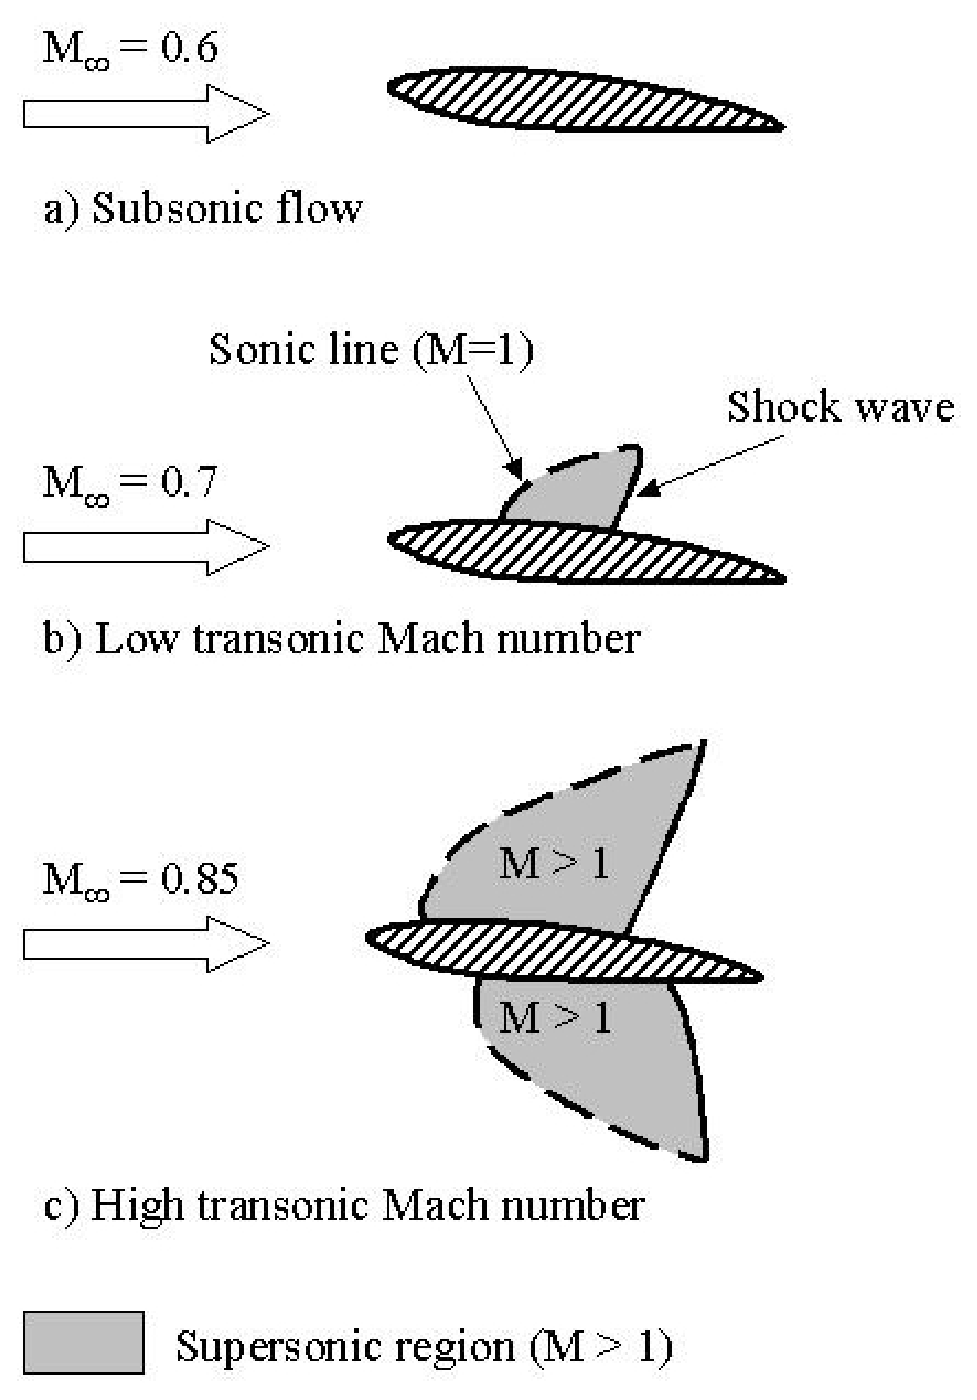
\includegraphics[height=6in]{aflow}
%     \else
%       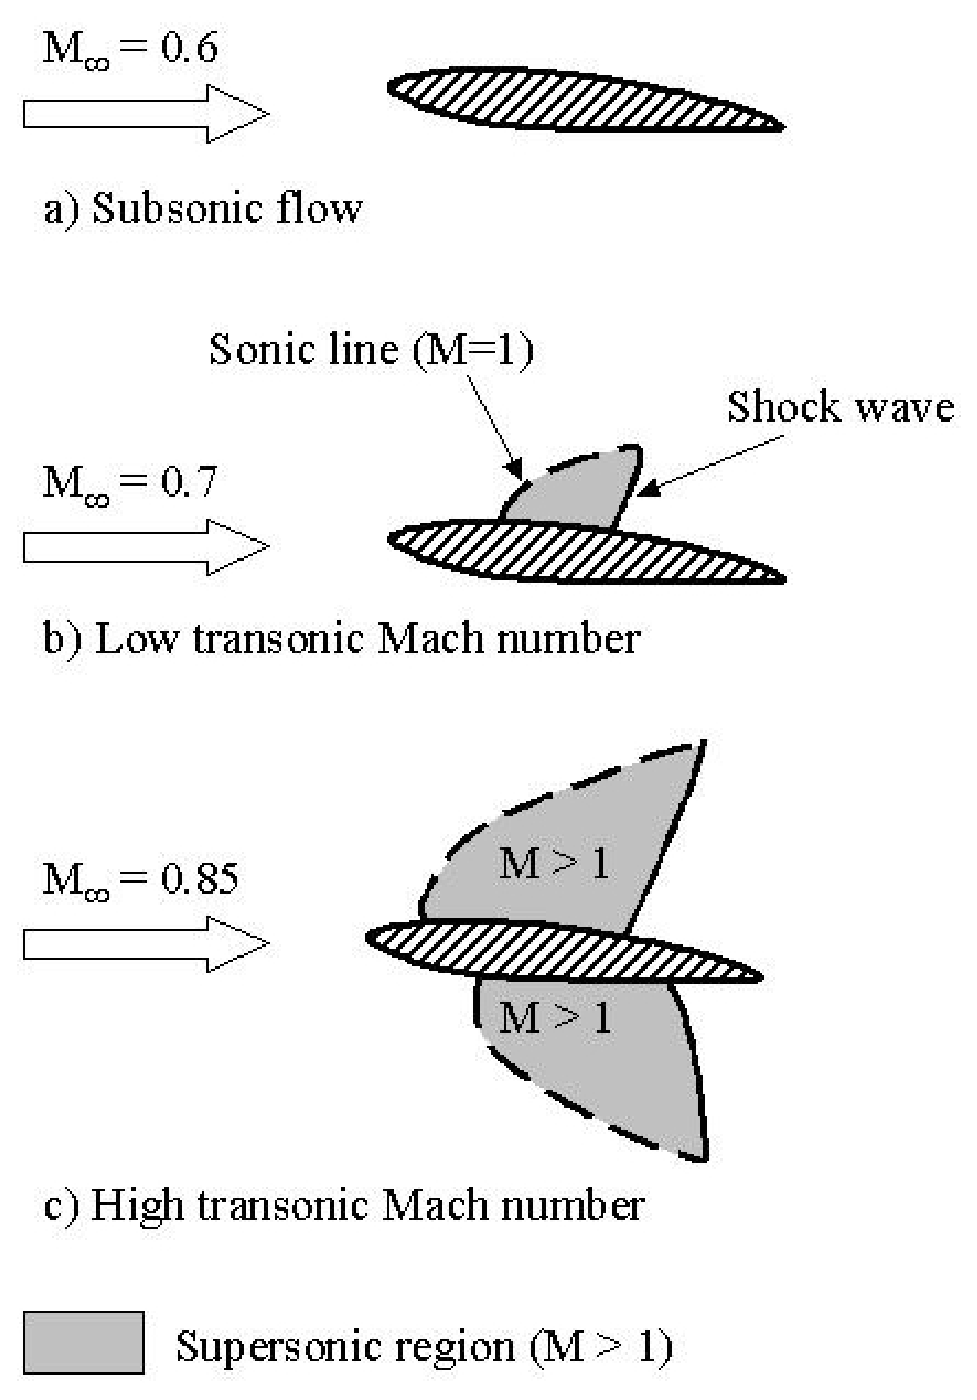
\includegraphics[bb = 92 86 545 742, height=6in]{aflow}
%     \fi
%     \caption{Airfoil Picture}
%     \label{FigAir}
%   \end{center}
% \end{figure}

% above code has been macro-fied in Classes/MacroFile.tex file
%\InsertFig{\IncludeGraphicsH{aflow}{6in}{92 86 545 742}}{Airfoil Picture}{FigAir}

% So as we have now labelled it we can reference it, like so (\ref{FigAir}) and it
% is on Page \pageref{FigAir}. And as we can see, it is a very nice picture and we
% can talk about it all we want and when we are tired we can move on to the next
% chapter ...

% I would also like to add an extra bookmark in acroread like so ...
% \ifpdf
%   \pdfbookmark[2]{bookmark text is here}{And this is what I want bookmarked}
% \fi
% ------------------------------------------------------------------------


%%% Local Variables: 
%%% mode: latex
%%% TeX-master: "../thesis"
%%% End: 

\chapter{Childline}
\ifpdf
    \graphicspath{{Chapter2/Chapter2Figs/PNG/}{Chapter2/Chapter2Figs/PDF/}{Chapter2/Chapter2Figs/}}
\else
    \graphicspath{{Chapter2/Chapter2Figs/EPS/}{Chapter2/Chapter2Figs/}}
\fi

\section{About Childline}
\markboth{\MakeUppercase{\thechapter. My Second Chapter }}
And now I begin my second chapter here ...

\section{Involvement of Synergy Sansthan}
\markboth{\MakeUppercase{\thechapter. My Second Chapter }}
and here I write more ...

\section{Some case studies}
\subsection{Jalim Singh}

\subsection{Vivek}

% \subsection{first subsection in the Second Section}
% ... and some more ...

% \subsection{second subsection in the Second Section}
% ... and some more ...

% \subsection{third subsection in the Second Section}
% ... and some more ...


% ------------------------------------------------------------------------

%%% Local Variables: 
%%% mode: latex
%%% TeX-master: "../thesis"
%%% End: 

\chapter{Entrepreneurship Development Program}
\ifpdf
    \graphicspath{{Chapter3/Chapter3Figs/PNG/}{Chapter3/Chapter3Figs/PDF/}{Chapter3/Chapter3Figs/}}
\else
    \graphicspath{{Chapter3/Chapter3Figs/EPS/}{Chapter3/Chapter3Figs/}}
\fi

\section{About}
Entrepreneurship Development Program was started at Synergy Sansthan with the help of ``Pravah'', a NGO based in Delhi. As the name suggests, it is related to developing entrepreneurial skills in individuals. 

\subsection{Goals}
The goals of EDP are to equip small and medium scale entrepreneurs with the skills needed to make their business bloom. To help them in procuring loans from the bank rather than from money lenders who would extort them. To make them independent eventually by making their business profitable for them.

\subsection{Methods}
The applicants would be given training on different aspects of business management. They would be told about how to maximize their profits and ubderstand their shortcomings. Apart from the analysis, Synergy Sansthan would Help in making all the proper paper work of the individuals. This would allow them to get loans from the bank at proper interest rates. A sustainable model would also be set up for them so that they can grow better.
% \subsubsection{first subsub section in the second subsection}
% ... and some more in the first subsub section otherwise it all looks the same
% doesn't it? well we can add some text to it ...

% \subsection{third subsection in the First Section}
% ... and some more ...

% \subsubsection{first subsub section in the third subsection}
% ... and some more in the first subsub section otherwise it all looks the same
% doesn't it? well we can add some text to it and some more and some more and
% some more and some more and some more and some more and some more ...

% \subsubsection{second subsub section in the third subsection}
% ... and some more in the first subsub section otherwise it all looks the same
% doesn't it? well we can add some text to it ...

\section{Mobilizing Strategies}
% \markboth{\MakeUppercase{\thechapter. My Third Chapter }}{\thechapter. My Third Chapter}
The mobilization strategy consisted of 5 steps as follows:
\begin{enumerate}
	\item \textbf{Mind Jog} \newline
		Ask them the goal of their life.
	\item \textbf{Personal Connection} \newline
		Ask the individual why did he start the business.
	\item \textbf{Information Exchange} \newline
		Tell them that India has 40-45\% youth and only 3\% of them get jobs. 
	\item \textbf{Information Application} \newline
		Tell them about the EDP.
	\item \textbf{Real World Connection} \newline
		Tell them the benefits of EDP and everything it has to offer.
\end{enumerate}

\section{Case Study}

\subsection{Rajiv Jat - Photocopy shop}
Rajiv Jat ran a small photocopy shop in Harda city. His daily business was of Rs. 150. He faced a lot of difficulty in supporting his family. Synergy Sansthan helped him out in setting his business properly. They got him a loan so that he could purchase 1 computer for his shop and get Internet access. This allowed him to have a small cyber-cafe. This enhanced his business considerably as the number of people having Internet access in Harda were very few.

% ------------------------------------------------------------------------


%%% Local Variables: 
%%% mode: latex
%%% TeX-master: "../thesis"
%%% End: 

% \chapter{Asha Training and NRHM}
\ifpdf
    \graphicspath{{Chapter2/Chapter2Figs/PNG/}{Chapter2/Chapter2Figs/PDF/}{Chapter2/Chapter2Figs/}}
\else
    \graphicspath{{Chapter2/Chapter2Figs/EPS/}{Chapter2/Chapter2Figs/}}
\fi

\section{About Asha training}
\markboth{\MakeUppercase{\thechapter. My Second Chapter }}
And now I begin my second chapter here ...

\section{About NRHM}
\markboth{\MakeUppercase{\thechapter. My Second Chapter }}
and here I write more ...

\section{Examples}

% \subsection{first subsection in the Second Section}
% ... and some more ...

% \subsection{second subsection in the Second Section}
% ... and some more ...

% \subsection{third subsection in the Second Section}
% ... and some more ...


% ------------------------------------------------------------------------

%%% Local Variables: 
%%% mode: latex
%%% TeX-master: "../thesis"
%%% End: 

\chapter{Positive Changes}
\ifpdf
    \graphicspath{{Chapter2/Chapter2Figs/PNG/}{Chapter2/Chapter2Figs/PDF/}{Chapter2/Chapter2Figs/}}
\else
    \graphicspath{{Chapter2/Chapter2Figs/EPS/}{Chapter2/Chapter2Figs/}}
\fi

\section{In child line}
\markboth{\MakeUppercase{\thechapter. My Second Chapter }}
And now I begin my second chapter here ...

\section{In villages}
\markboth{\MakeUppercase{\thechapter. My Second Chapter }}
and here I write more ...

\section{In EDP}

% \subsection{first subsection in the Second Section}
% ... and some more ...

% \subsection{second subsection in the Second Section}
% ... and some more ...

% \subsection{third subsection in the Second Section}
% ... and some more ...


% ------------------------------------------------------------------------

%%% Local Variables: 
%%% mode: latex
%%% TeX-master: "../thesis"
%%% End: 

\chapter{Negative things}
\ifpdf
    \graphicspath{{Chapter2/Chapter2Figs/PNG/}{Chapter2/Chapter2Figs/PDF/}{Chapter2/Chapter2Figs/}}
\else
    \graphicspath{{Chapter2/Chapter2Figs/EPS/}{Chapter2/Chapter2Figs/}}
\fi

\section{Low awareness}
\markboth{\MakeUppercase{\thechapter. My Second Chapter }}
And now I begin my second chapter here ...

\section{Employees}
\markboth{\MakeUppercase{\thechapter. My Second Chapter }}
and here I write more ...

% \subsection{first subsection in the Second Section}
% ... and some more ...

% \subsection{second subsection in the Second Section}
% ... and some more ...

% \subsection{third subsection in the Second Section}
% ... and some more ...


% ------------------------------------------------------------------------

%%% Local Variables: 
%%% mode: latex
%%% TeX-master: "../thesis"
%%% End: 

\def\baselinestretch{1}
\chapter{Conclusions}
\ifpdf
    \graphicspath{{Conclusions/ConclusionsFigs/PNG/}{Conclusions/ConclusionsFigs/PDF/}{Conclusions/ConclusionsFigs/}}
\else
    \graphicspath{{Conclusions/ConclusionsFigs/EPS/}{Conclusions/ConclusionsFigs/}}
\fi

\def\baselinestretch{1.66}

Synergy Sansthan is a very young and interesting NGO. It has a different ideology as compared from other NGOs. It has produced a lot of results as well.

\vspace{1cm}

The most striking fact that I liked was the policy of the creators that they would all leave the NGO at the age of 35 and not stay on the board or be in any official way related to it. This will ensure that the NGO stays an NGO for the youth and takes more and more action. It will not become a dynastic NGO which is run for profit.


\vspace{1cm}
As it is targeting the youth, it is able to deliver maximum amount of change. By organizing workshops in colleges in Harda the issues of the youth are directly faced and resolved.

\vspace{1cm}

Synergy Sansthan should be given more opportunities and allowed to grow more. Its scope right now is limited to a few districts in Madhya Pradesh. If this increases then the amount of change that it can deliver will be monumental.
%%% ----------------------------------------------------------------------

% ------------------------------------------------------------------------

%%% Local Variables: 
%%% mode: latex
%%% TeX-master: "../thesis"
%%% End: 


\backmatter % book mode only
\appendix
\chapter{Overall experience}

\vspace{0cm}

My overall experience from this exercise has been very enlightening. I have become aware on a lot of issues which I didn't know about.

I got in touch with people from different people and had interesting conversations with them. 

I learned quite a few new things which I wouldn't have the chance to otherwise like:
\begin{enumerate}
\item When we try to solve any issue, we should not give a solution directly. We should consider all of its adversities before arriving at a decision otherwise our effort can have a negative effect.
\item To bring change, everyone has to change: adolescents, youth, adults, senior citizens. All the cogs of the clock have to function for it to show the right time. Even if one is malfunctioning, the entire balance is destroyed.
\item To help the society one must not necessarily have to go in the social service world but must try to bring some changes in himself.
\item We often dismiss social issues blaming the government, the system, the officials etc. but that in no way helps in solving them or giving a solution. We should try to put ourselves in the shoes of the person facing the difficulty and then consider trying to give a solution.
\end{enumerate}

I would definitely like to take part in another activity of this sort.
% ------------------------------------------------------------------------

%%% Local Variables: 
%%% mode: latex
%%% TeX-master: "../thesis"
%%% End: 

% \chapter{Appdx B}

and here I put some more postamble ...

% ------------------------------------------------------------------------

%%% Local Variables: 
%%% mode: latex
%%% TeX-master: "../thesis"
%%% End: 


\bibliographystyle{plainnat}
%\bibliographystyle{Classes/CUEDbiblio}
%\bibliographystyle{Classes/jmb}
%\bibliographystyle{Classes/jmb} % bibliography style
% \renewcommand{\bibname}{References} % changes default name Bibliography to References
% \bibliography{References/references} % References file

\end{document}
